% STATUS: ACTIVE -- SSOT for the Form B (unknown wall position) w-axis
%          gain-law derivation.  Equation-only house style; every remark,
%          rationale and provenance lives in formB_ws_ref.tex (same section
%          numbers).  Main file covers S1-S8 (the scope of the companion
%          documents); S9-S11 (filter equations, seeds/priors, acceptance)
%          live as notes in formB_ws_ref.tex (user decision 2026-07-31).
%          Parameter order everywhere: b_w, p_w, w_s (user, 2026-07-31).
% ======================================================
% Compile: xelatex formB_ws.tex
% Path:    reference/eq17_analysis/derivation/formB_ws.tex
% Companion: formB_ws_ref.tex (appendix: conventions, rationale, provenance)
% ======================================================

\documentclass[11pt,a4paper,fontset=none]{ctexart}

\usepackage[fleqn]{amsmath}
\usepackage{amssymb,bm}
\setlength{\mathindent}{0pt}
\usepackage{geometry}
\geometry{margin=2.0cm}
\usepackage{graphicx}

\setlength{\parindent}{0pt}
\setlength{\parskip}{0.80em}
\linespread{1.08}
\setlength{\emergencystretch}{2em}
\setlength{\abovedisplayskip}{10pt}
\setlength{\belowdisplayskip}{10pt}

\begin{document}

\section{Gain law}

(bars denote normalized quantities: lengths by $R$, $\bar{a} = a/a_o$,
$\bar{f} = a_o f$;
$\bar{w} > \bar{w}_s$, $b > 0$, $p > 0$;
$e_{\theta} = \theta - \hat{\theta}$)

\begin{align*}
\bar{a}(\bar{w}-\bar{w}_s,\, b,\, p)
  &= 1 - \Bigl(1 + \frac{\bar{w}-\bar{w}_s}{b}\Bigr)^{-p}
  \qquad (\bar{w}_s - 1:\ \text{unknown surface position}) \\
\bar{a}(\bar{w}-\bar{w}_s,\, b_w,\, p_w)
  &= 1 - \Bigl(1 + \frac{\bar{w}-\bar{w}_s}{b_w}\Bigr)^{-p_w} \\
\bar{a}\bigl(\bar{w}_d-\hat{\bar{w}}_s,\, \hat{b}_w,\, \hat{p}_w\bigr)
  &= 1 - \Bigl(1 + \frac{\bar{w}_d-\hat{\bar{w}}_s}{\hat{b}_w}\Bigr)^{-\hat{p}_w}
\end{align*}

\begin{equation*}
a_w = a_o\,\bar{a}(\bar{w}-\bar{w}_s,\, b_w,\, p_w),
\qquad a_o = \frac{\Delta t}{\gamma_N R}
\quad \text{($a_o$ fixed, not a state)}
\end{equation*}

\begin{equation*}
p = 1:\qquad
\bar{a} = \frac{\bar{w}-\bar{w}_s}{(\bar{w}-\bar{w}_s) + b},
\qquad
\frac{d\bar{a}}{d\bar{w}} = \frac{b}{\bigl((\bar{w}-\bar{w}_s)+b\bigr)^{2}}
\end{equation*}

\textbf{Parallel-axis law}\quad (2026-08-02, Stage 1a.  The $x/y$ truth
$c_\parallel$ leaves contact with Goldman log behavior --- no family
member reproduces it, and the best representation places its origin
INSIDE the wall: the parallel axes cannot report the physical wall.
Constants derived at init from the planned envelope (offline
truth-curve fit, the envelope-prior mechanism); the $x/y$ filters lock
$(b, p, \bar{w}_s)$ and consume the SHARED wall estimate one-way from
the $z$ filter; rationale, widths and health record in ref)

\begin{align*}
\bar{a}_\parallel
  &= 1 - \Bigl(1 +
    \frac{\bar{w} - (\hat{\bar{w}}_{s,z} + \Delta_\parallel)}
         {b_\parallel}\Bigr)^{-p_\parallel},
\qquad
\Delta_\parallel := \bar{w}_{s0,\parallel} - 1 \\
(b_\parallel,\ p_\parallel,\ \bar{w}_{s0,\parallel})
  &= \arg\min\ \sup_{\text{envelope}}
    \bigl|\bar{a}_\parallel - 1/c_\parallel\bigr|
  = (0.5217,\ 0.9770,\ 0.5918)
\quad (\sup\ 0.038\%)
\end{align*}

\begin{align*}
P_{\bar{a}\bar{a},\parallel}[0] &= (\text{shape floor}_\parallel)^2, \\
\text{floor}_\parallel
  &= \sqrt{\textstyle\sup^2_{fit} + (\sup\bar{a}'\,\delta_{w_{s0}})^2
    + (\sup|\tfrac{g}{b}\bar{a}'|\,\delta_b)^2
    + (\sup|(1{-}\bar{a})\ln(1{+}\tfrac{g}{b})|\,\delta_p)^2}
  = 0.0052
\end{align*}

(boundary widths $\delta_{b},\delta_{p},\delta_{w_{s0}}
= 0.0104,\ 0.0061,\ 0.0147$ --- floor $\pm 0.1$ / ceiling refits;
the $z$ law and the $z$ filter are untouched)

\section{Gain rate and parameter Jacobians}

\begin{align*}
\bar{a}'(\bar{w}-\bar{w}_s,\, b,\, p)
  &:= \frac{d\bar{a}}{d\bar{w}}
   = \frac{p}{b}\,\Bigl(1 + \frac{\bar{w}-\bar{w}_s}{b}\Bigr)^{-p-1} \\
\bar{a}'\bigl(\bar{w}_d-\hat{\bar{w}}_s,\, \hat{b}_w,\, \hat{p}_w\bigr)
  &= \frac{\hat{p}_w}{\hat{b}_w}\,
     \Bigl(1 + \frac{\bar{w}_d-\hat{\bar{w}}_s}{\hat{b}_w}\Bigr)^{-\hat{p}_w-1}
\end{align*}

\begin{equation*}
\frac{\partial \bar{a}}{\partial \bar{w}_s} = -\,\bar{a}'
\qquad \text{(exact, any $b$, $p$)}
\end{equation*}

\begin{align*}
&\bar{a}'(\bar{w}_d-\bar{w}_s,\, b_w,\, p_w)
 - \bar{a}'\bigl(\bar{w}_d-\hat{\bar{w}}_s,\, \hat{b}_w,\, \hat{p}_w\bigr) \\
&\qquad = J_b\bigl(\bar{w}_d-\hat{\bar{w}}_s, \hat{b}_w, \hat{p}_w\bigr)\,e_{b_w}
 + J_p\bigl(\bar{w}_d-\hat{\bar{w}}_s, \hat{b}_w, \hat{p}_w\bigr)\,e_{p_w}
 + J_{w_s}\bigl(\bar{w}_d-\hat{\bar{w}}_s, \hat{b}_w, \hat{p}_w\bigr)\,e_{\bar{w}_s}
\end{align*}

\begin{align*}
J_b\bigl(\bar{w}_d-\hat{\bar{w}}_s, \hat{b}_w, \hat{p}_w\bigr)
  &= \Bigl[-\frac{1}{\hat{b}_w}
     + \frac{(\hat{p}_w+1)\,(\bar{w}_d-\hat{\bar{w}}_s)}
            {\hat{b}_w\bigl((\bar{w}_d-\hat{\bar{w}}_s)+\hat{b}_w\bigr)}\Bigr]\,
     \bar{a}'\bigl(\bar{w}_d-\hat{\bar{w}}_s, \hat{b}_w, \hat{p}_w\bigr) \\
J_p\bigl(\bar{w}_d-\hat{\bar{w}}_s, \hat{b}_w, \hat{p}_w\bigr)
  &= \Bigl[\frac{1}{\hat{p}_w}
     - \ln\Bigl(1 + \frac{\bar{w}_d-\hat{\bar{w}}_s}{\hat{b}_w}\Bigr)\Bigr]\,
     \bar{a}'\bigl(\bar{w}_d-\hat{\bar{w}}_s, \hat{b}_w, \hat{p}_w\bigr) \\
J_{w_s}\bigl(\bar{w}_d-\hat{\bar{w}}_s, \hat{b}_w, \hat{p}_w\bigr)
  &= \Bigl[\frac{\hat{p}_w+1}
            {(\bar{w}_d-\hat{\bar{w}}_s)+\hat{b}_w}\Bigr]\,
     \bar{a}'\bigl(\bar{w}_d-\hat{\bar{w}}_s, \hat{b}_w, \hat{p}_w\bigr)
\end{align*}

\section{True dynamics}

$\bigl(\delta\bar{w}_j[k] := \delta\bar{w}[k-d+j-1],\ \ j = 1,\dots,d{+}1,
\ \ d = 2;\qquad \delta\bar{w}_D \equiv 0 \ \text{hereafter}\bigr)$

\begin{align*}
\bar{w}[k] &= \bar{w}_d[k] - \delta\bar{w}_3[k] \\
\bar{a}_w[k+1] &= \bar{a}_w\bigl(\bar{w}[k+1]\bigr)
  = \bar{a}\bigl(\bar{w}_d[k+1]-\bar{w}_s-\delta\bar{w}_3[k+1],\, b_w,\, p_w\bigr) \\
\bar{w}_d[k+1] &= \bar{w}_d[k] + \Delta\bar{w}_d[k]
\end{align*}

\begin{align*}
\delta\bar{w}_1[k+1] &= \delta\bar{w}_2[k] \\
\delta\bar{w}_2[k+1] &= \delta\bar{w}_3[k] \\
\delta\bar{w}_3[k+1] &= \lambda_c\,\delta\bar{w}_3[k]
  - F_{dw}[k]\,e_{\bar{a}_w}[k] - \varepsilon_w[k]
  \qquad (e_{\bar{a}_w} = \bar{a}_w - \hat{\bar{a}}_w) \\
b_w[k+1] &= b_w[k] \\
p_w[k+1] &= p_w[k] \\
\bar{w}_s[k+1] &= \bar{w}_s[k]
\end{align*}
\begin{align*}
F_{dw}[k] &:= \bar{f}_{dw}[k] + (1-\lambda_c)\sum_{i=1}^{d} \bar{f}_{dw}[k-i] \\
\varepsilon_w[k] &:= \bar{a}_w[k]\bar{f}_T[k]
  + (1-\lambda_c)\sum_{i=1}^{d} \bar{a}_w[k-i]\bar{f}_T[k-i]
  - (1-\lambda_c)\,n_w[k-d]
\end{align*}

(sign and lag of the $n_w$ feedthrough corrected 2026-08-01 by log
forensics --- regression tap $-0.296$ at $k{-}d$; the former
$+(1-\lambda_c)n_w[k]$ leaves the variance unchanged, see ref)

\section{Process model}

\begin{align*}
\bar{w}[k+1] - \bar{w}[k]
  &= \Delta\bar{w}_d[k] + (1-\lambda_c)\,\delta\bar{w}_3[k]
   + F_{dw}[k]\,e_{\bar{a}_w}[k] + \varepsilon_w[k]
\end{align*}

\begin{align*}
\bar{a}_w[k+1] = \bar{a}_w[k] + \bar{a}'[k]\,\Bigl[
  \Delta\bar{w}_d[k] + (1-\lambda_c)\,\delta\bar{w}_3[k]
  + F_{dw}[k]\,e_{\bar{a}_w}[k] + \varepsilon_w[k] \Bigr]
\end{align*}
\begin{equation*}
\bar{a}'[k] = \bar{a}'\bigl(\bar{w}_d[k]-\bar{w}_s[k],\, b_w[k],\, p_w[k]\bigr)
\end{equation*}

\begin{equation*}
\mathbf{x}[k] = \bigl[\,\delta\bar{w}_1,\ \delta\bar{w}_2,\ \delta\bar{w}_3,\
\bar{a}_w,\ b_w,\ p_w,\ \bar{w}_s\,\bigr]^{\top}[k] \qquad (d = 2)
\end{equation*}

\begin{align*}
\delta\bar{w}_1[k+1] &= \delta\bar{w}_2[k] \\
\delta\bar{w}_2[k+1] &= \delta\bar{w}_3[k] \\
\delta\bar{w}_3[k+1] &= \lambda_c\,\delta\bar{w}_3[k]
  - F_{dw}[k]\,e_{\bar{a}_w}[k] - \varepsilon_w[k] \\
\bar{a}_w[k+1] &= \bar{a}_w[k] + \bar{a}'[k]\,\Bigl[
  \Delta\bar{w}_d[k] + (1-\lambda_c)\,\delta\bar{w}_3[k]
  + F_{dw}[k]\,e_{\bar{a}_w}[k] + \varepsilon_w[k] \Bigr] \\
b_w[k+1] &= b_w[k] \\
p_w[k+1] &= p_w[k] \\
\bar{w}_s[k+1] &= \bar{w}_s[k]
\end{align*}

\section{Estimator}

\begin{align*}
\delta\hat{\bar{w}}_1[k+1] &= \delta\hat{\bar{w}}_2[k] \\
\delta\hat{\bar{w}}_2[k+1] &= \delta\hat{\bar{w}}_3[k] \\
\delta\hat{\bar{w}}_3[k+1] &= \lambda_c\,\delta\hat{\bar{w}}_3[k] \\
\hat{\bar{a}}_w[k+1] &= \hat{\bar{a}}_w[k] + \hat{\bar{a}}'[k]\,\Bigl[
  \Delta\bar{w}_d[k] + (1-\lambda_c)\,\delta\hat{\bar{w}}_3[k] \Bigr] \\
\hat{b}_w[k+1] &= \hat{b}_w[k] \\
\hat{p}_w[k+1] &= \hat{p}_w[k] \\
\hat{\bar{w}}_s[k+1] &= \hat{\bar{w}}_s[k]
\end{align*}
\begin{equation*}
\hat{\bar{a}}'[k] = \bar{a}'\bigl(\bar{w}_d[k]-\hat{\bar{w}}_s[k],\,
\hat{b}_w[k],\, \hat{p}_w[k]\bigr)
\end{equation*}

\section{Error dynamics}

(True $-$ Estimator; coefficients at the estimate)

\begin{equation*}
e_{\delta\bar{w}_j} = \delta\bar{w}_j - \delta\hat{\bar{w}}_j
\ \ (j = 1,2,3),
\qquad
\mathbf{e} = \bigl[\,e_{\delta\bar{w}_1},\ e_{\delta\bar{w}_2},\
e_{\delta\bar{w}_3},\ e_{\bar{a}_w},\ e_{b_w},\ e_{p_w},\
e_{\bar{w}_s}\,\bigr]^{\top}
\end{equation*}

\begin{align*}
e_{\delta\bar{w}_1}[k+1] &= e_{\delta\bar{w}_2}[k] \\
e_{\delta\bar{w}_2}[k+1] &= e_{\delta\bar{w}_3}[k] \\
e_{\delta\bar{w}_3}[k+1] &= \lambda_c\,e_{\delta\bar{w}_3}[k]
  - F_{dw}[k]\,e_{\bar{a}_w}[k] - \varepsilon_w[k] \\
e_{\bar{a}_w}[k+1]
  &= \bigl[1 + \hat{\bar{a}}'[k]\,F_{dw}[k]\bigr]\,e_{\bar{a}_w}[k]
   + J_{b_w}[k]\bigl[\Delta\bar{w}_d[k]
     + (1-\lambda_c)\,\delta\hat{\bar{w}}_3[k]\bigr]\,e_{b_w}[k] \\
  &\quad + J_{p_w}[k]\bigl[\Delta\bar{w}_d[k]
     + (1-\lambda_c)\,\delta\hat{\bar{w}}_3[k]\bigr]\,e_{p_w}[k]
   + J_{w_s}[k]\bigl[\Delta\bar{w}_d[k]
     + (1-\lambda_c)\,\delta\hat{\bar{w}}_3[k]\bigr]\,e_{\bar{w}_s}[k] \\
  &\quad + (1-\lambda_c)\,\hat{\bar{a}}'[k]\,e_{\delta\bar{w}_3}[k]
   + \hat{\bar{a}}'[k]\,\varepsilon_w[k] \\
e_{b_w}[k+1] &= e_{b_w}[k] \\
e_{p_w}[k+1] &= e_{p_w}[k] \\
e_{\bar{w}_s}[k+1] &= e_{\bar{w}_s}[k]
\end{align*}

\begin{align*}
J_{b_w}[k] &= J_b\bigl(\bar{w}_d[k]-\hat{\bar{w}}_s[k],\,
  \hat{b}_w[k],\, \hat{p}_w[k]\bigr) \\
J_{p_w}[k] &= J_p\bigl(\bar{w}_d[k]-\hat{\bar{w}}_s[k],\,
  \hat{b}_w[k],\, \hat{p}_w[k]\bigr) \\
J_{w_s}[k] &= J_{w_s}\bigl(\bar{w}_d[k]-\hat{\bar{w}}_s[k],\,
  \hat{b}_w[k],\, \hat{p}_w[k]\bigr)
\end{align*}

\begin{equation*}
\mathbf{e}[k+1] = \mathbf{F}_e[k]\,\mathbf{e}[k] + \mathbf{q}[k]
\end{equation*}

{\small
\setlength{\arraycolsep}{3pt}
\begin{equation*}
\mathbf{F}_e[k] =
\begin{bmatrix}
0 & 1 & 0 & 0 & 0 & 0 & 0 \\
0 & 0 & 1 & 0 & 0 & 0 & 0 \\
0 & 0 & \lambda_c & -F_{dw} & 0 & 0 & 0 \\
0 & 0 & (1{-}\lambda_c)\hat{\bar{a}}' & 1{+}\hat{\bar{a}}'F_{dw} &
J_{b_w}\bigl[\Delta\bar{w}_d{+}(1{-}\lambda_c)\delta\hat{\bar{w}}_3\bigr] &
J_{p_w}\bigl[\Delta\bar{w}_d{+}(1{-}\lambda_c)\delta\hat{\bar{w}}_3\bigr] &
J_{w_s}\bigl[\Delta\bar{w}_d{+}(1{-}\lambda_c)\delta\hat{\bar{w}}_3\bigr] \\
0 & 0 & 0 & 0 & 1 & 0 & 0 \\
0 & 0 & 0 & 0 & 0 & 1 & 0 \\
0 & 0 & 0 & 0 & 0 & 0 & 1
\end{bmatrix}
\end{equation*}
}

\begin{equation*}
\mathbf{q}[k] = \bigl[\,0,\ 0,\ -\varepsilon_w[k],\
\hat{\bar{a}}'[k]\,\varepsilon_w[k],\ 0,\ 0,\ 0\,\bigr]^{\top}
\qquad \bigl(q_4 = -\hat{\bar{a}}'[k]\,q_3\bigr)
\end{equation*}

\section{Measurement and innovation}

\textbf{Measurement}\quad ($d$-step delay; $\bar{a}_{wm} = a_{wm}/a_o$;
$y_2$ raw readout --- AR(1) whitening enters with $R_2$, S8)

\begin{align*}
\nabla_d\bar{w}_d[k] &:= \bar{w}_d[k] - \bar{w}_d[k-d] \\
y_1[k] &= \delta\bar{w}_m[k] = \delta\bar{w}_1[k] + n_w[k] \\
y_2[k] &= \bar{a}_{wm}[k] = \bar{a}_w[k-d] + n_a[k]
\end{align*}

\textbf{Delay back-off}

\begin{align*}
\bar{a}_w[k-d]
  &= \bar{a}_w[k] - \bar{a}'[k]\,\nabla_d\bar{w}_d[k]
\qquad \Longrightarrow \qquad
y_2[k]
  = \bar{a}_w[k] - \bar{a}'[k]\,\nabla_d\bar{w}_d[k] + n_a[k]
\end{align*}

\textbf{Linearization}\quad (partials at the estimate; $\bar{a}'$ does not
depend on the state $\bar{a}_w$, so $\partial y_2/\partial\bar{a}_w$ is
exactly $1$)

\begin{align*}
\frac{\partial y_2}{\partial \bar{a}_w} &= 1, \qquad
\frac{\partial y_2}{\partial b_w}
  = -\nabla_d\bar{w}_d[k]\,J_{b_w}[k], \qquad
\frac{\partial y_2}{\partial p_w}
  = -\nabla_d\bar{w}_d[k]\,J_{p_w}[k], \qquad
\frac{\partial y_2}{\partial \bar{w}_s}
  = -\nabla_d\bar{w}_d[k]\,J_{w_s}[k]
\end{align*}

\textbf{Output equation}\quad ($\mathbf{H}$ is the Jacobian; row 2 is
nonlinear in $\mathbf{x}$, so $\mathbf{H}\mathbf{x}$ is its linearization,
not an identity)

\begin{align*}
\mathbf{y}[k] = \mathbf{H}[k]\,\mathbf{x}[k] + \mathbf{r}[k],
\qquad
\mathbf{r}[k] =
\begin{bmatrix} n_w[k] \\ n_a[k] \end{bmatrix}
\end{align*}

{\small
\setlength{\arraycolsep}{4pt}
\begin{equation*}
\mathbf{H}[k] =
\begin{bmatrix}
1 & 0 & 0 & 0 & 0 & 0 & 0 \\
0 & 0 & 0 & 1 &
-\nabla_d\bar{w}_d\,J_{b_w} &
-\nabla_d\bar{w}_d\,J_{p_w} &
-\nabla_d\bar{w}_d\,J_{w_s}
\end{bmatrix}
\end{equation*}
}

\textbf{Innovation}

\begin{align*}
e_{y_1}[k] &= y_1[k] - \delta\hat{\bar{w}}_1[k]
  = e_{\delta\bar{w}_1}[k] + n_w[k] \\
e_{y_2}[k] &= y_2[k] - \hat{\bar{a}}_w[k]
  + \hat{\bar{a}}'[k]\,\nabla_d\bar{w}_d[k] \\
  &= e_{\bar{a}_w}[k]
  - \nabla_d\bar{w}_d[k]\,
    \bigl[J_{b_w}[k]\,e_{b_w}[k] + J_{p_w}[k]\,e_{p_w}[k]
    + J_{w_s}[k]\,e_{\bar{w}_s}[k]\bigr]
  + n_a[k]
\end{align*}

\section{Process and measurement noise}

\textbf{Process noise $Q$}\quad (full $\mathrm{Var}(\varepsilon_w)$
container --- thermal history and $n_w$ feedthrough included, only the
cross-step correlations of $\varepsilon_w$ dropped; revision 2026-08-01,
supersedes the current-step-only container; see ref)

\begin{align*}
q_3[k] &= -\bar{a}_w[k]\,\bar{f}_T[k], \qquad
q_4[k] = \hat{\bar{a}}'[k]\,\bar{a}_w[k]\,\bar{f}_T[k]
       = -\hat{\bar{a}}'[k]\,q_3[k] \\
\gamma(\bar{w}) &= \gamma_N\,c(\bar{w}), \qquad
\sigma^2_{\bar{f}_T} = a_o^2\,\frac{4k_BT\,\gamma(\bar{w})}{\Delta t},
\qquad
\bar{a}_w = \frac{\Delta t}{a_o\,\gamma(\bar{w})\,R}
\quad\Longrightarrow\quad
\mathrm{Var}\bigl(\bar{a}_w\bar{f}_T\bigr)
  = \frac{4k_BT\,a_o}{R}\,\bar{a}_w
\end{align*}

\begin{align*}
Q_{33}[k]
  &= \mathrm{Var}(\varepsilon_w[k])
   = \frac{4k_BT\,a_o}{R}\,
     \Bigl(\bar{a}_w[k]
     + (1-\lambda_c)^2\sum_{i=1}^{d}\bar{a}_w[k-i]\Bigr)
   + (1-\lambda_c)^2\,\sigma^2_{n_w} \\
Q_{34}[k] &= Q_{43}[k] = -\hat{\bar{a}}'[k]\,Q_{33}[k], \qquad
Q_{44}[k] = \hat{\bar{a}}'[k]^{2}\,Q_{33}[k]
\end{align*}
\begin{equation*}
Q_{55} = Q_{66} = Q_{77} = 0 \quad
(b_w,\ p_w,\ \bar{w}_s\ \text{constant})
\end{equation*}

All other entries vanish; the gain block is rank one, since
$q_4 = -\hat{\bar{a}}'[k]\,q_3$.  (run time: entries at the current
estimate)

\textbf{Measurement noise $R = \mathrm{diag}(R_1, R_2)$}\quad
($a_{cov}$ = EWMA coefficient, $IF_{var}$ = MA($d$) inflation factor of
$\hat{\sigma}^2_{\delta\bar{w}_r}$; $y_2$ treated as white here ---
whitened treatment in the ref notes)

\begin{equation*}
R_1 = \sigma^2_{n_w}
\end{equation*}

\begin{align*}
\sigma^2_{\delta\bar{w}_r}[k]
  &= C_{dpmr}\,\frac{4k_BT\,a_o}{R}\,\bar{a}_w[k] + C_n\,\sigma^2_{n_w}
   = C_{dpmr}\,\frac{4k_BT\,a_o}{R}\,\bigl(\bar{a}_w[k] + \xi\bigr) \\
\xi &:= \frac{C_n}{C_{dpmr}}\,\frac{\sigma^2_{n_w}}{4k_BT\,a_o/R} \\
\bar{a}_{wm}[k]
  &= \frac{\hat{\sigma}^2_{\delta\bar{w}_r}[k] - C_n\,\sigma^2_{n_w}}
          {C_{dpmr}\,\bigl(4k_BT\,a_o/R\bigr)} \\
\mathrm{Var}\bigl(\hat{\sigma}^2_{\delta\bar{w}_r}\bigr)
  &= K_{var}\,IF_{var}\,\bigl(\sigma^2_{\delta\bar{w}_r}\bigr)^{2},
\qquad
K_{var} = \frac{2a_{cov}}{2-a_{cov}}
\end{align*}

\begin{equation*}
R_2[k] = K_{var}\,IF_{var}\,\bigl(\bar{a}_w[k]+\xi\bigr)^{2}
  + d\,Q_{44}[k]
\end{equation*}

($C_{dpmr}$, $C_n$: \texttt{Cdpmr\_Cn\_derivation.tex} --- stationary,
noise-only derivation; the former ``defect 2'' motion excess was RETRACTED
2026-08-01 ($N{=}48$: $+1.33\%$ n.s.); see ref)

\textbf{MA(2) augmentation}\quad (2026-08-01; supersedes the white
container above.  $\varepsilon_w$ is MA(2) across steps --- the $d$-step
loop delay makes consecutive $\varepsilon_w$ share thermal kicks; the
white container matches the per-step variance but understates the
zero-frequency power by $(1+2(1{-}\lambda_c))^2/(1+2(1{-}\lambda_c)^2)
= 2.17$ at $\lambda_c = 0.7$; verification and ablation in ref)

\begin{align*}
m_1[k] &:= \bar{a}_w[k-1]\bar{f}_T[k-1], \qquad
m_2[k] := \bar{a}_w[k-2]\bar{f}_T[k-2] \\
\varepsilon_w[k] &= \bar{a}_w[k]\bar{f}_T[k]
  + (1-\lambda_c)\bigl(m_1[k] + m_2[k]\bigr)
  - (1-\lambda_c)\,n_w[k-d] \\
m_1[k+1] &= \bar{a}_w[k]\bar{f}_T[k], \qquad
m_2[k+1] = m_1[k]
\end{align*}

\begin{equation*}
\mathbf{x} \to
\bigl[\,\mathbf{x},\ m_1,\ m_2\,\bigr]^{\top}
\qquad (9\ \text{states; } m_1, m_2\ \text{at slots } 8, 9)
\end{equation*}

\begin{align*}
\mathbf{F}_e(3,8) &= \mathbf{F}_e(3,9) = -(1-\lambda_c), \qquad
\mathbf{F}_e(4,8) = \mathbf{F}_e(4,9) = \hat{\bar{a}}'[k]\,(1-\lambda_c), \\
\mathbf{F}_e(8,\cdot) &= \mathbf{0}, \qquad
\mathbf{F}_e(9,8) = 1
\qquad (\text{rows } 1\text{--}7\ \text{otherwise unchanged})
\end{align*}

\textbf{Per-step noise}\quad (white by construction; the off-diagonal
couplings $Q_{38}$, $Q_{48}$ are load-bearing --- a diagonal $Q$ gives
$C(1) = (1-\lambda_c)^2\sigma^2_T$, $C(2) = 0$, wrong)

\begin{align*}
\mathbf{g}_T &= \bigl[\,0,\ 0,\ -1,\ \hat{\bar{a}}'[k],\ 0,\ 0,\ 0,\
  1,\ 0\,\bigr]^{\top}, \qquad
\mathbf{g}_n = (1-\lambda_c)\bigl[\,0,\ 0,\ -1,\ \hat{\bar{a}}'[k],\
  0,\ 0,\ 0,\ 0,\ 0\,\bigr]^{\top} \\
\mathbf{Q}[k] &= \frac{4k_BT\,a_o}{R}\,\bar{a}_w[k]\,
  \mathbf{g}_T\mathbf{g}_T^{\top}
  + \sigma^2_{n_w}\,\mathbf{g}_n\mathbf{g}_n^{\top}
\qquad (\text{rank } 2)
\end{align*}

\textbf{Autocovariance identity}\quad ($\alpha := 1-\lambda_c$,
$\sigma^2_T := (4k_BT a_o/R)\,\bar{a}_w$; the augmented model reproduces
exactly, the white container only $C(0)$)

\begin{align*}
C(0) &= (1+2\alpha^2)\,\sigma^2_T + \alpha^2\sigma^2_{n_w}, \qquad
C(1) = \alpha(1+\alpha)\,\sigma^2_T, \qquad
C(2) = \alpha\,\sigma^2_T, \qquad C(j\geq3) = 0 \\
S(0) &= (1+2\alpha)^2\,\sigma^2_T + \alpha^2\sigma^2_{n_w}
\end{align*}

\textbf{Initialization}\quad ($m$-block from the same DARE pattern as
the position block, now $5\times5$ over
$[\delta\bar{w}_1\ \delta\bar{w}_2\ \delta\bar{w}_3\ m_1\ m_2]$;
$P_{m_1m_1}[0] = P_{m_2m_2}[0]$ carried by the DARE steady state at the
seed gain)

\textbf{$y_2$ self-echo correction}\quad (2026-08-01.  The variance
readout measures the ACTUAL loop, which runs on the applied gain
$\hat{\bar{a}}_{ctrl}$; a control-gain error shifts the loop pole and
the residual variance follows it with sensitivity $S$ --- the innovation
therefore carries only $(1{-}S)$ of the true-gain deviation, and the
uncorrected filter overcounts $y_2$ information by $1/(1{-}S)^2$ and
partially confirms its own error; verification in ref)

\begin{align*}
\sigma^2_{\delta\bar{w}_r}
  &= \sigma^2\bigl(\bar{a}_w,\ \hat{\bar{a}}_{ctrl}\bigr),
\qquad
S := \frac{\partial \ln \sigma^2_{\delta\bar{w}_r}}
          {\partial \ln \hat{\bar{a}}_{ctrl}} \\
E\bigl[y_2[k]\bigr]
  &= (1-S)\,\bar{a}_w[k-d] + S\,\hat{\bar{a}}_{ctrl}[k] + \ldots \\
\Longrightarrow\quad
\mathbf{H}_{2,:} &\to (1-S)\,\mathbf{H}_{2,:},
\qquad
y_{2,pred} = \hat{\bar{a}}_w - (1-S)\,\hat{\bar{a}}'\,\nabla_d\bar{w}_d
\end{align*}

\begin{equation*}
S = \frac{S_T\,\bar{a}_w + S_n\,\xi}{\bar{a}_w + \xi},
\qquad
S_T,\ S_n\ \text{from the exact 6-state Lyapunov covariance of the
mismatched loop}
\end{equation*}

($S_T$ far field $0.319$; paired-forcing measurement
$0.323 \pm 0.043$; $S(\bar{w})$ near-constant $0.310$--$0.319$ on the
envelope; $R_2$ unchanged --- the noise floor is on the actual variance
level)

\clearpage

\section*{Simulation figures}

(canonical scenario, $z$ axis; per panel: gain tracking, relative gain error,
free parameters)

\begin{center}
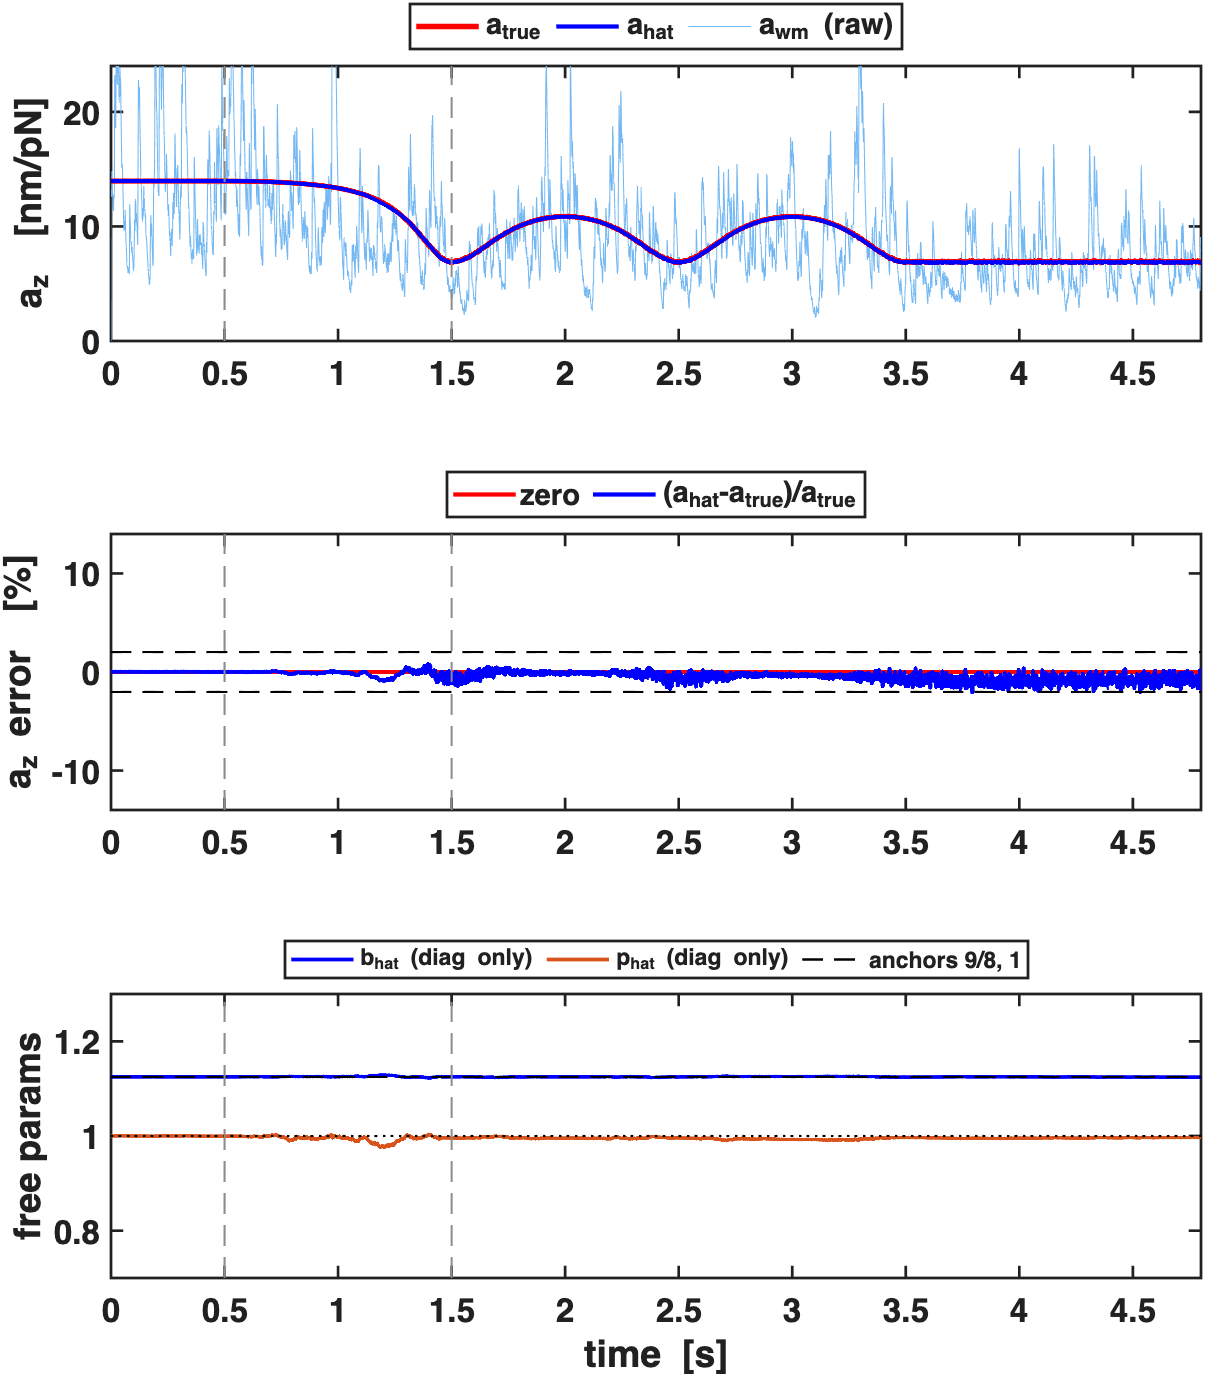
\includegraphics[width=0.49\linewidth]{figures/formB_c1_seed7.png}\hfill
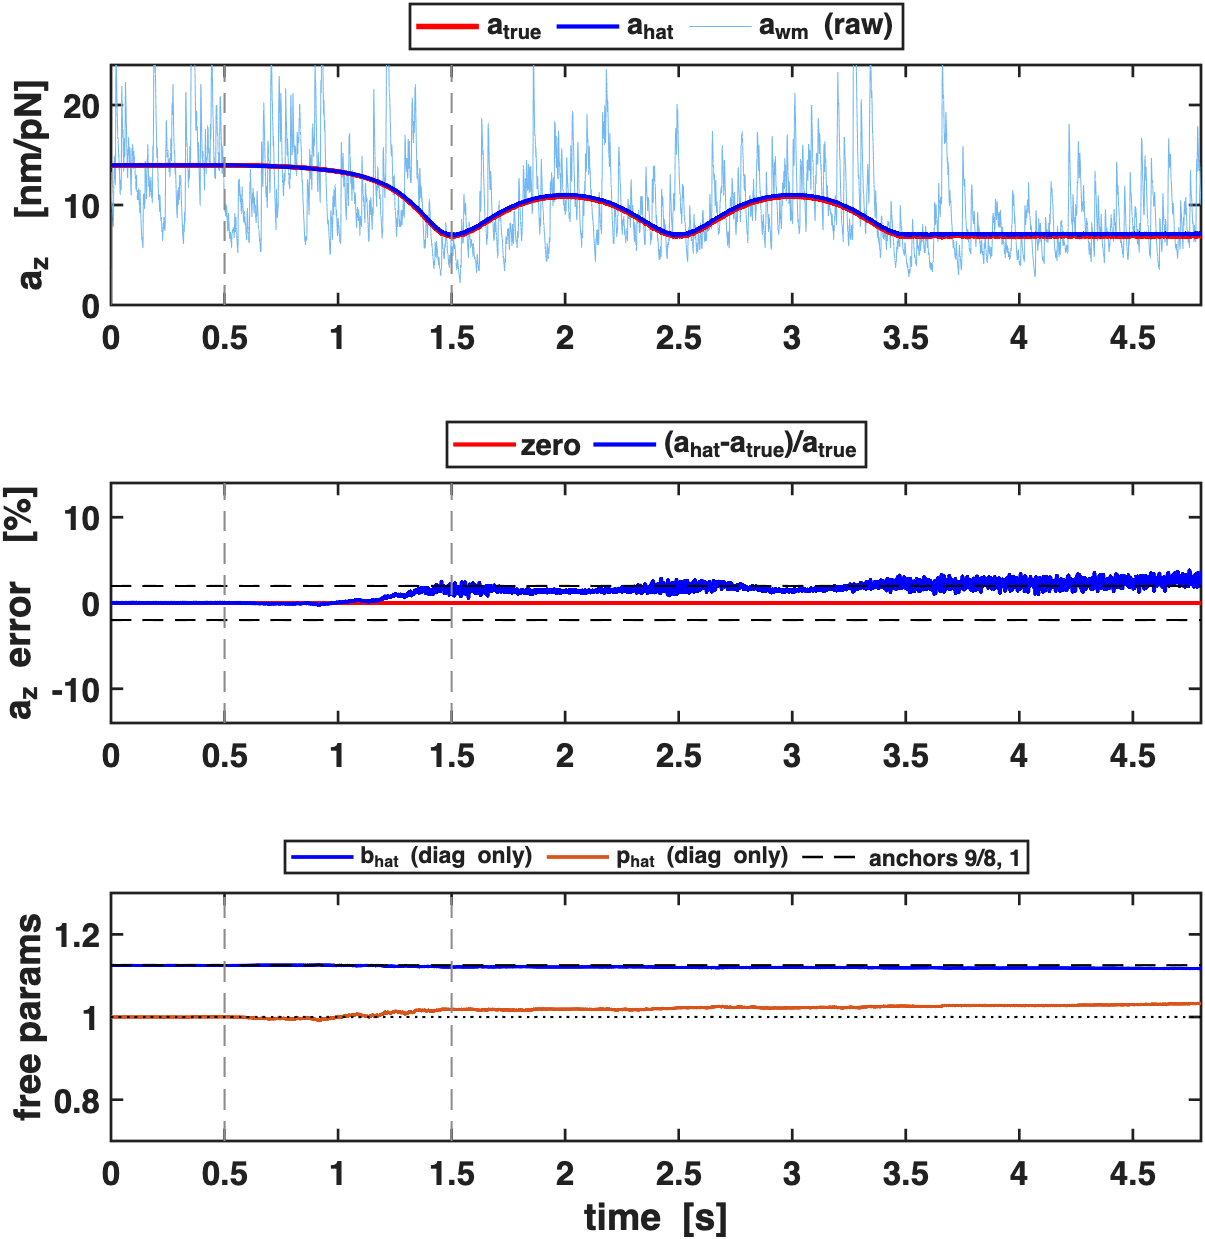
\includegraphics[width=0.49\linewidth]{figures/formB_c1_seed11.png}

Config 1 --- estimate $(b, p)$, $w_s$ locked at 1: seed 7 (left) vs seed 11 (right).
\end{center}

\clearpage

\begin{center}
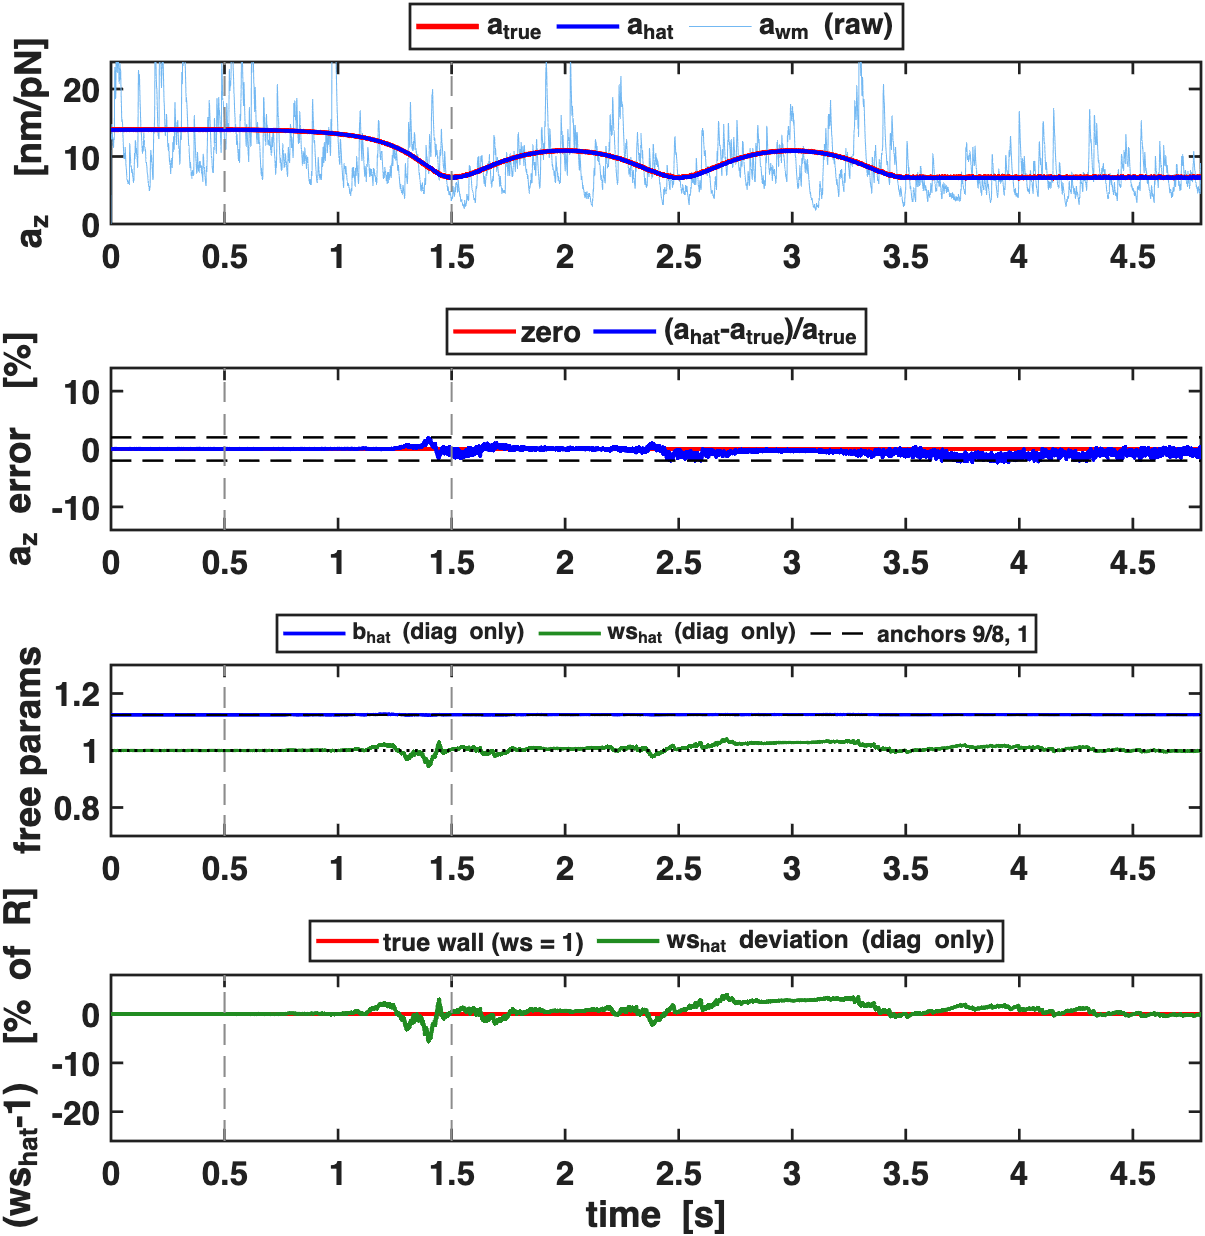
\includegraphics[width=0.49\linewidth]{figures/formB_c2_seed7.png}\hfill
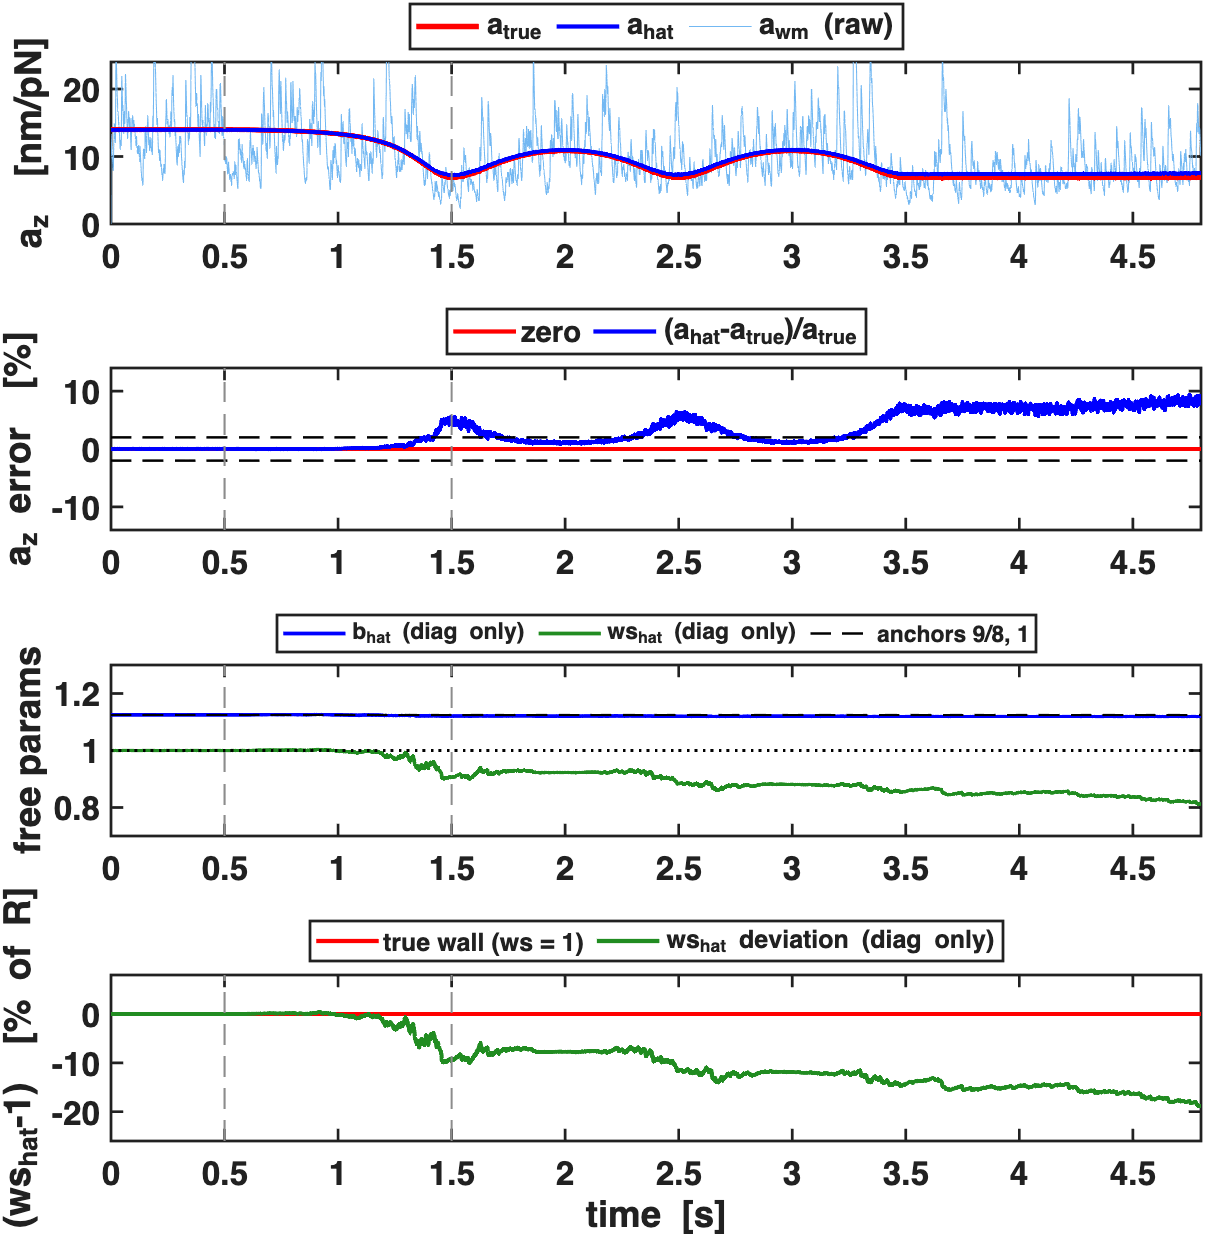
\includegraphics[width=0.49\linewidth]{figures/formB_c2_seed11.png}

Config 2 --- $p$ locked at 1, estimate $(b, w_s)$: seed 7 vs seed 11.
\end{center}

\clearpage

\begin{center}
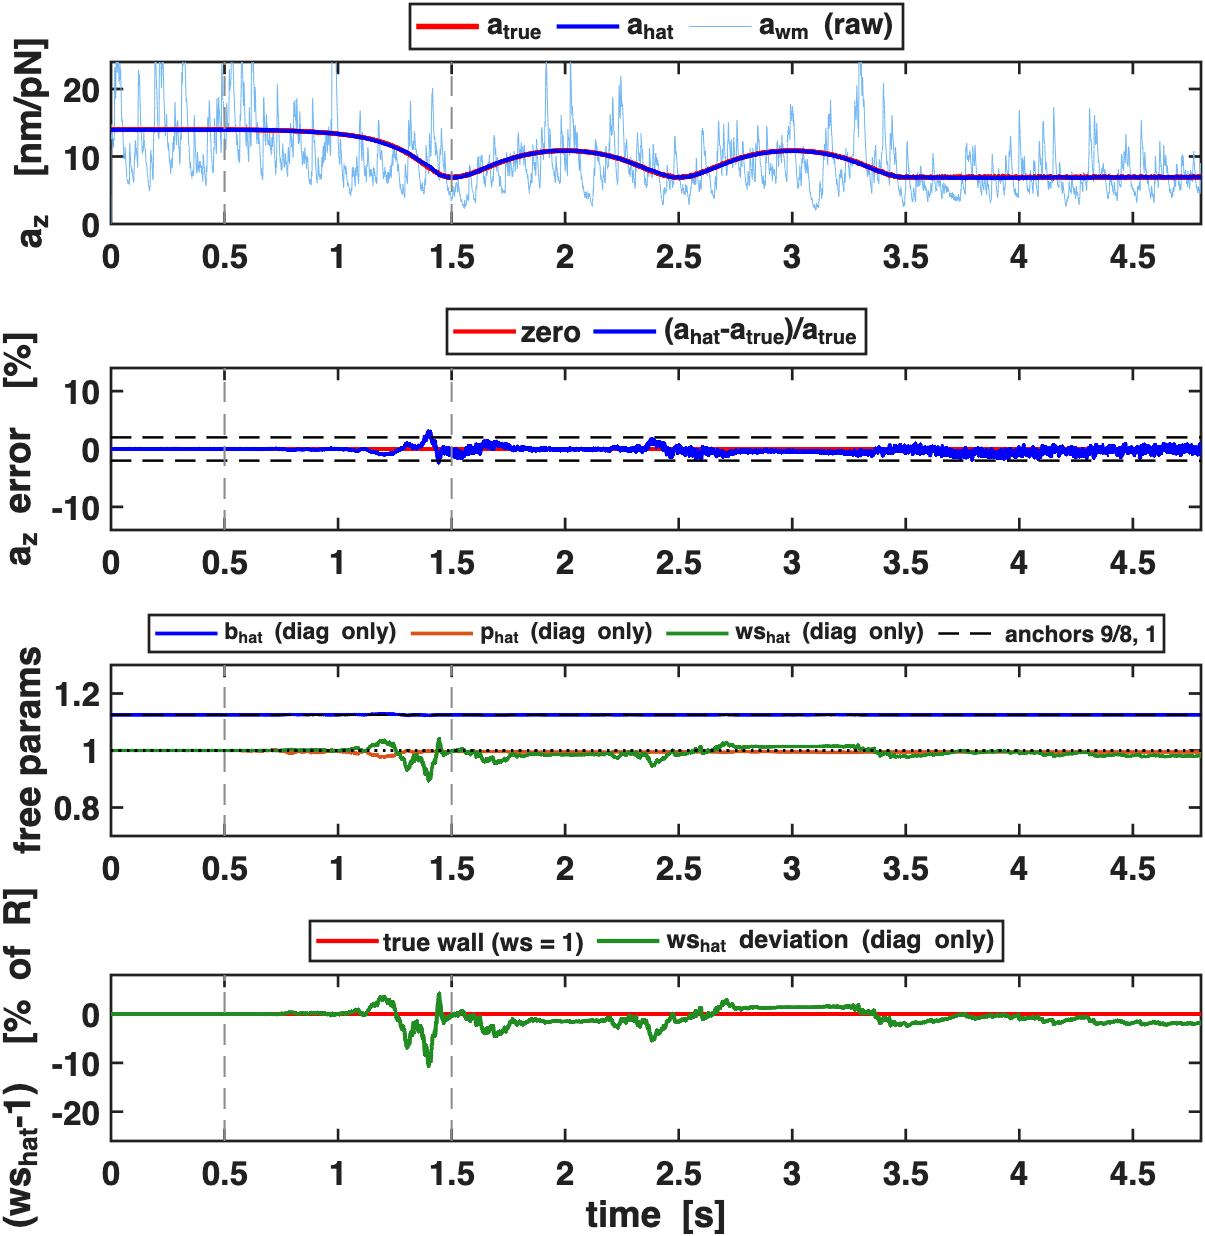
\includegraphics[width=0.49\linewidth]{figures/formB_c3_seed7.png}\hfill
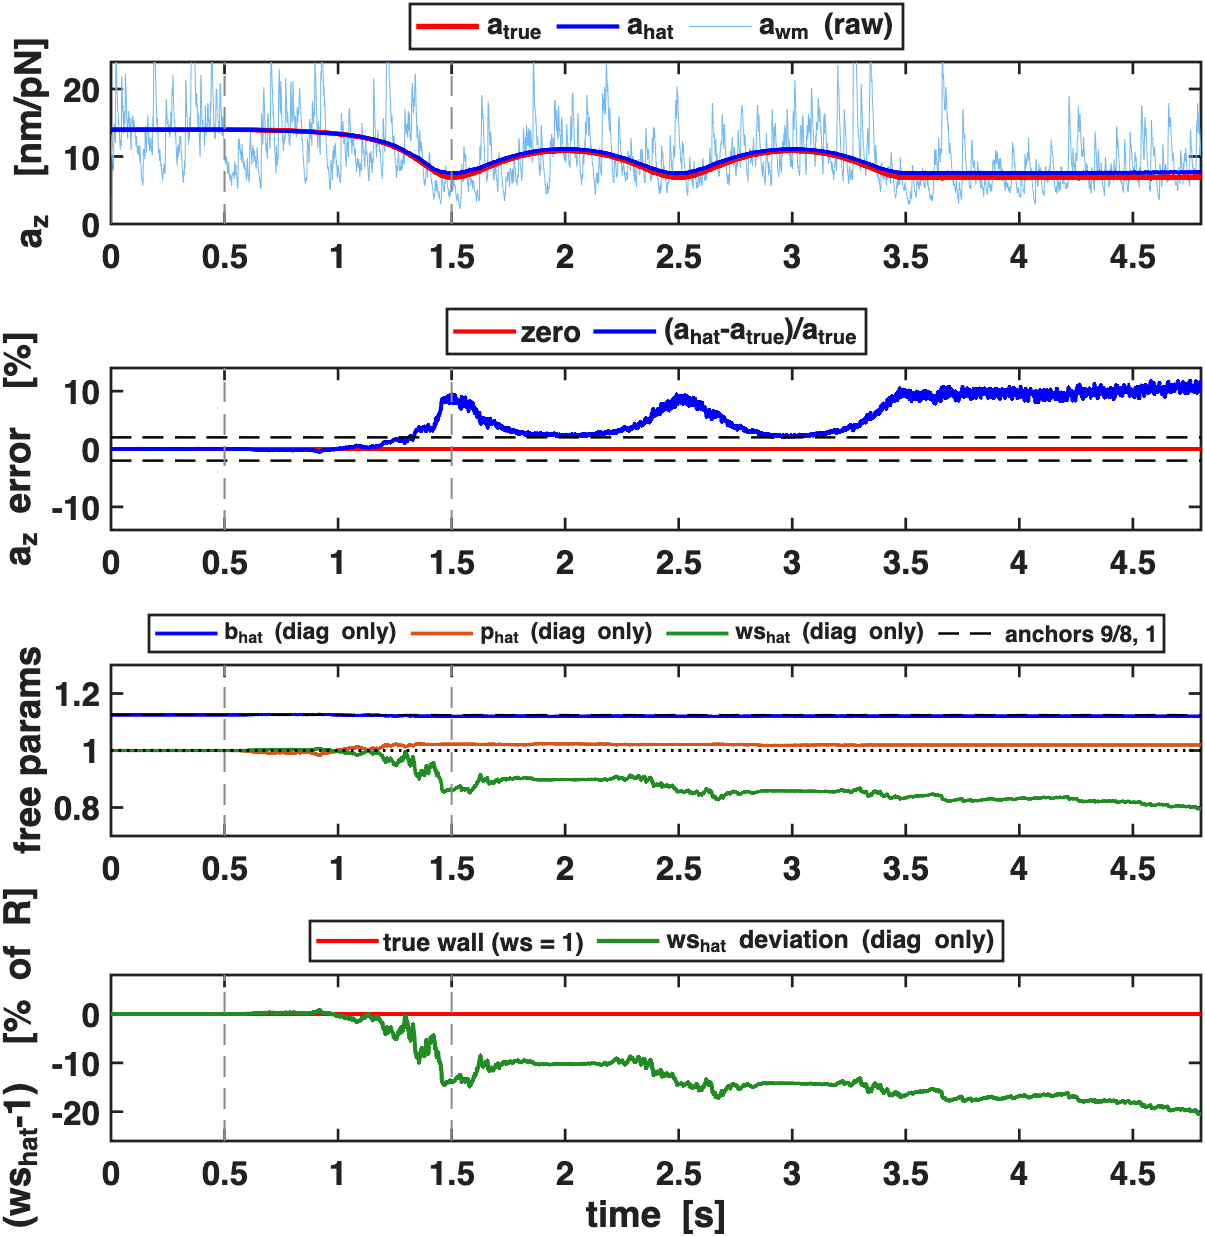
\includegraphics[width=0.49\linewidth]{figures/formB_c3_seed11.png}

Config 3 --- estimate $(b, p, w_s)$: seed 7 vs seed 11.
\end{center}

\clearpage

\begin{center}
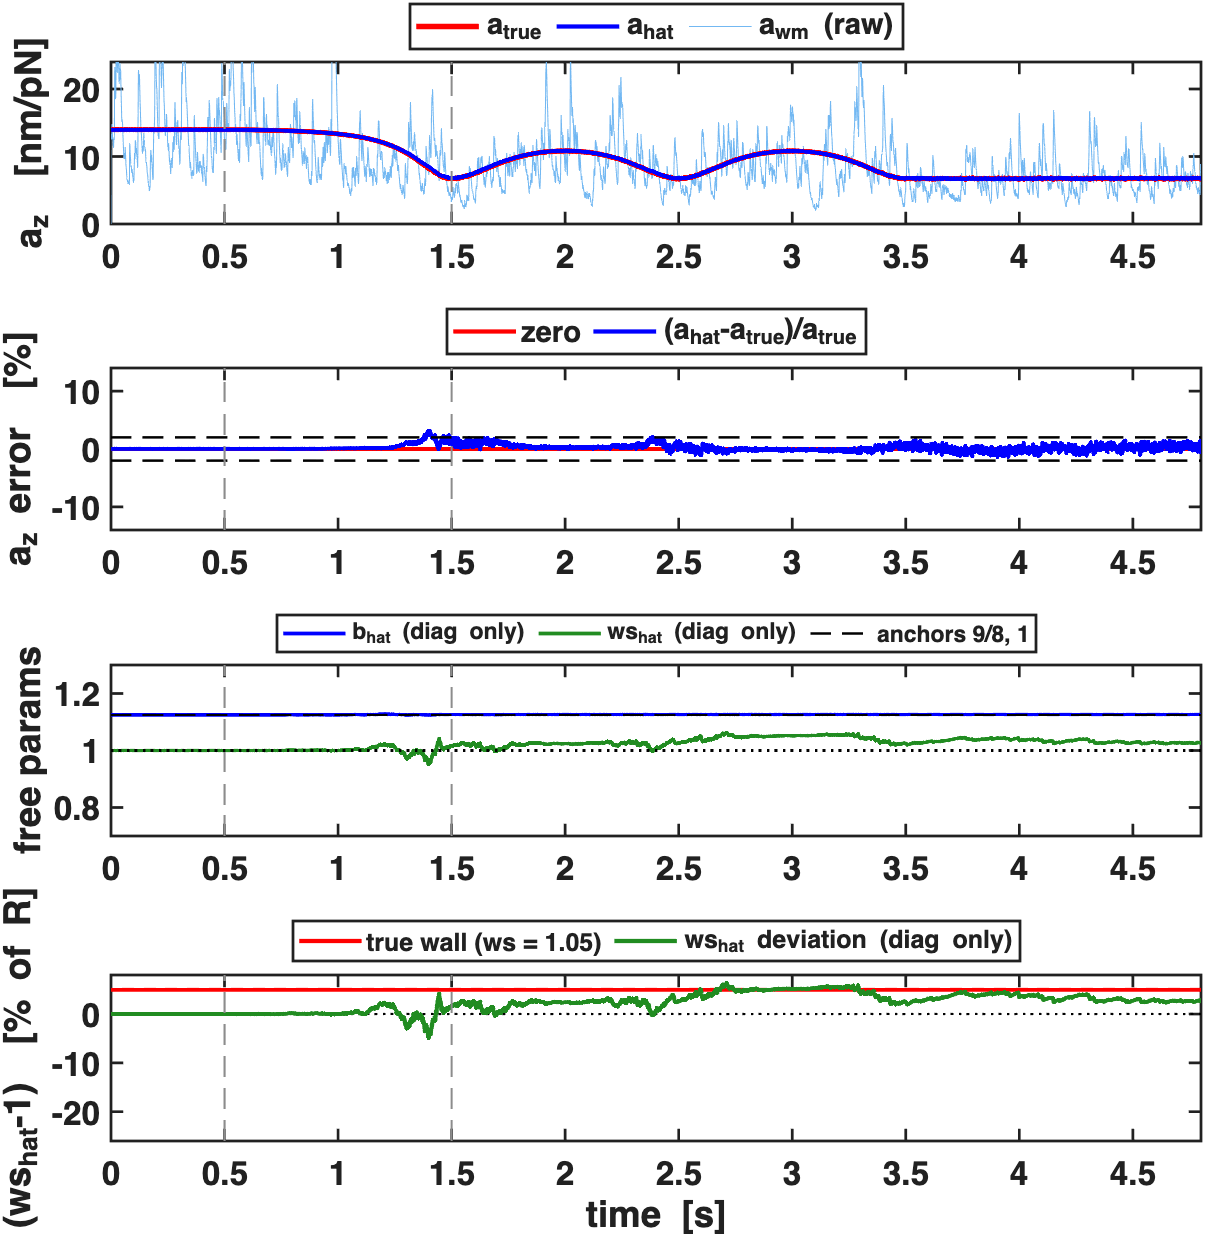
\includegraphics[width=0.49\linewidth]{figures/formB_c4_seed7.png}\hfill
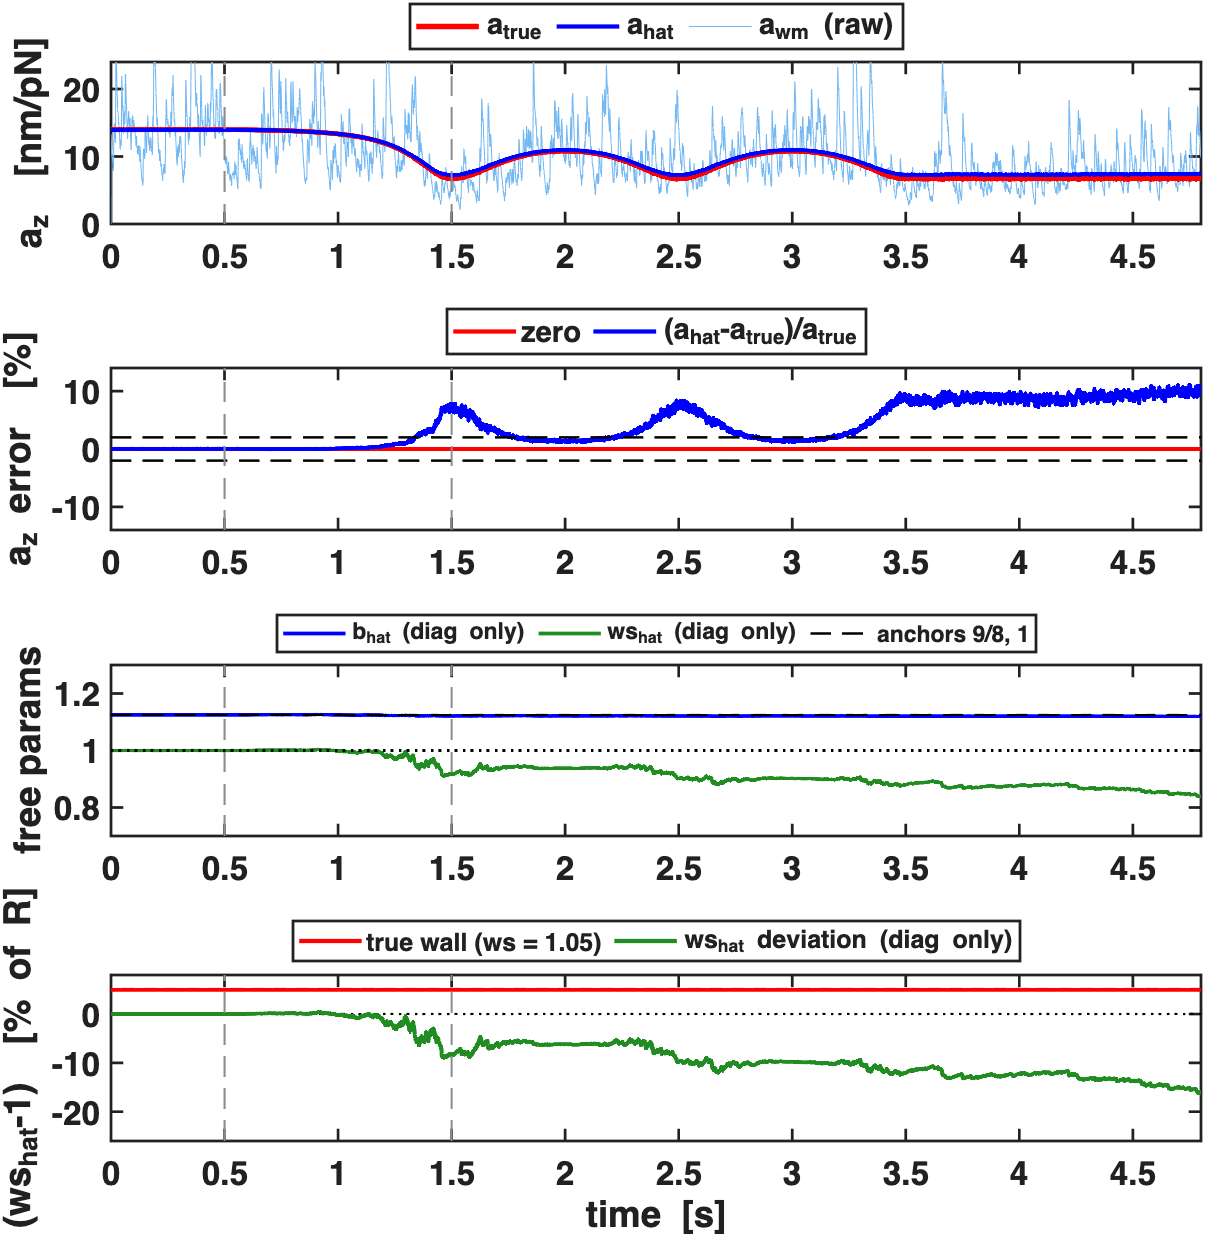
\includegraphics[width=0.49\linewidth]{figures/formB_c4_seed11.png}

Config 4 --- config 2 with the TRUE wall injected at $\bar{w}_s = 1.05$
(plant-side shift, S11 protocol): seed 7 vs seed 11.
\end{center}

\clearpage

\begin{center}
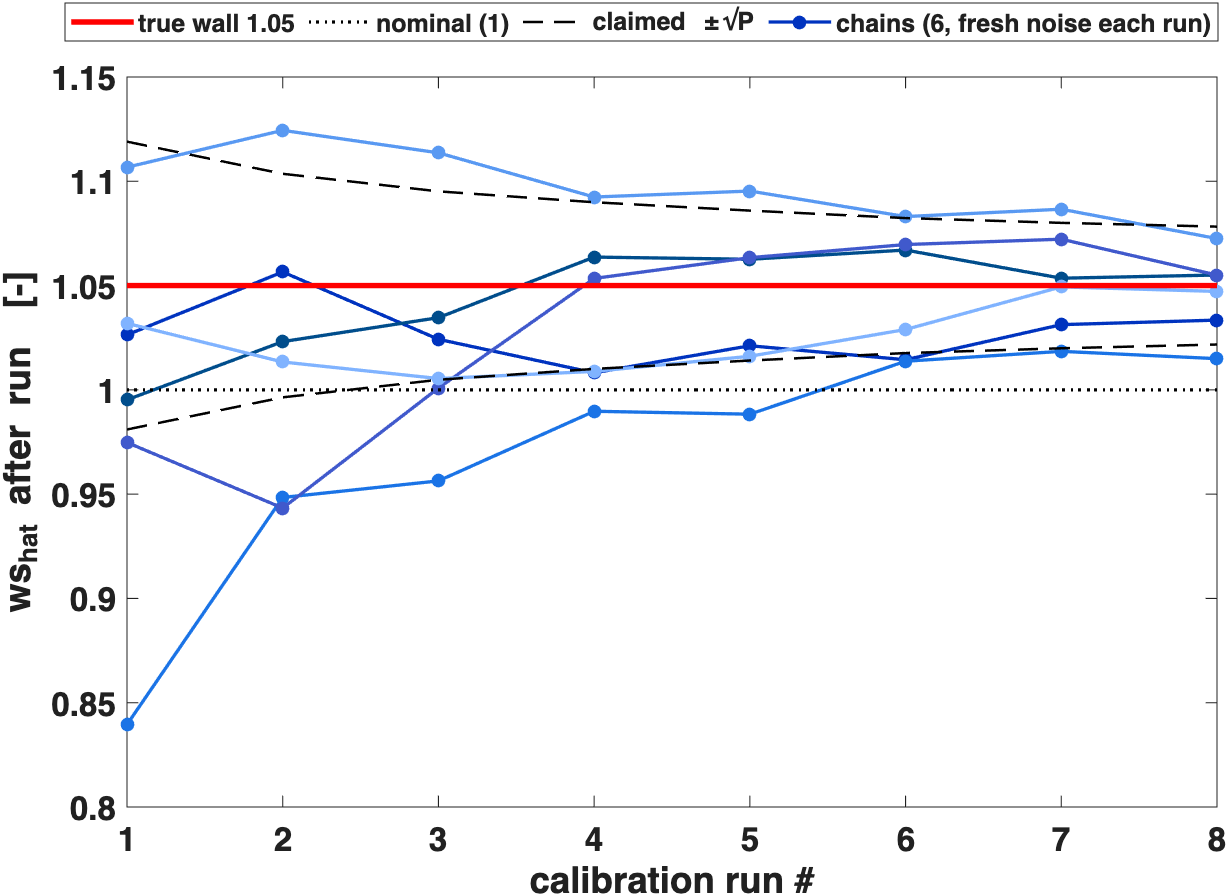
\includegraphics[width=0.49\linewidth]{figures/formB_c5_chain.png}\hfill
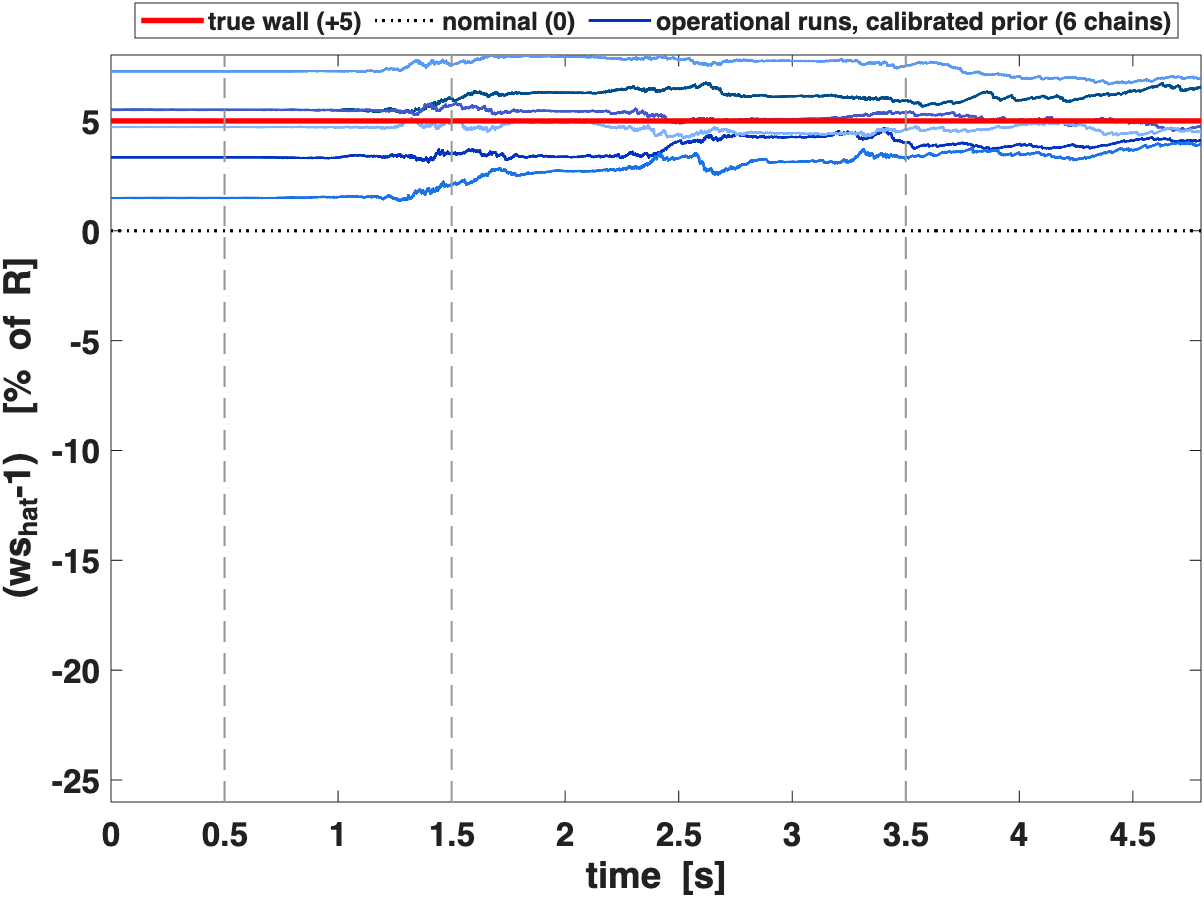
\includegraphics[width=0.49\linewidth]{figures/formB_c5_operational.png}

Config 5 --- $\bar{w}_s$ as a calibration constant: sequential posterior
handoff (run $n$'s $(\hat{\bar{w}}_s, \sqrt{P_{w_s}})$ = run $n{+}1$'s
prior), 6 chains $\times$ 8 runs, fresh noise each run, true wall $1.05$
(left); operational run on the calibrated prior --- cross-chain
$\hat{\bar{w}}_s$ error std $1.3\%$, descent peak $1.69\%$
($\approx$ the config-1 locked floor) (right).
\end{center}

\clearpage

\begin{center}
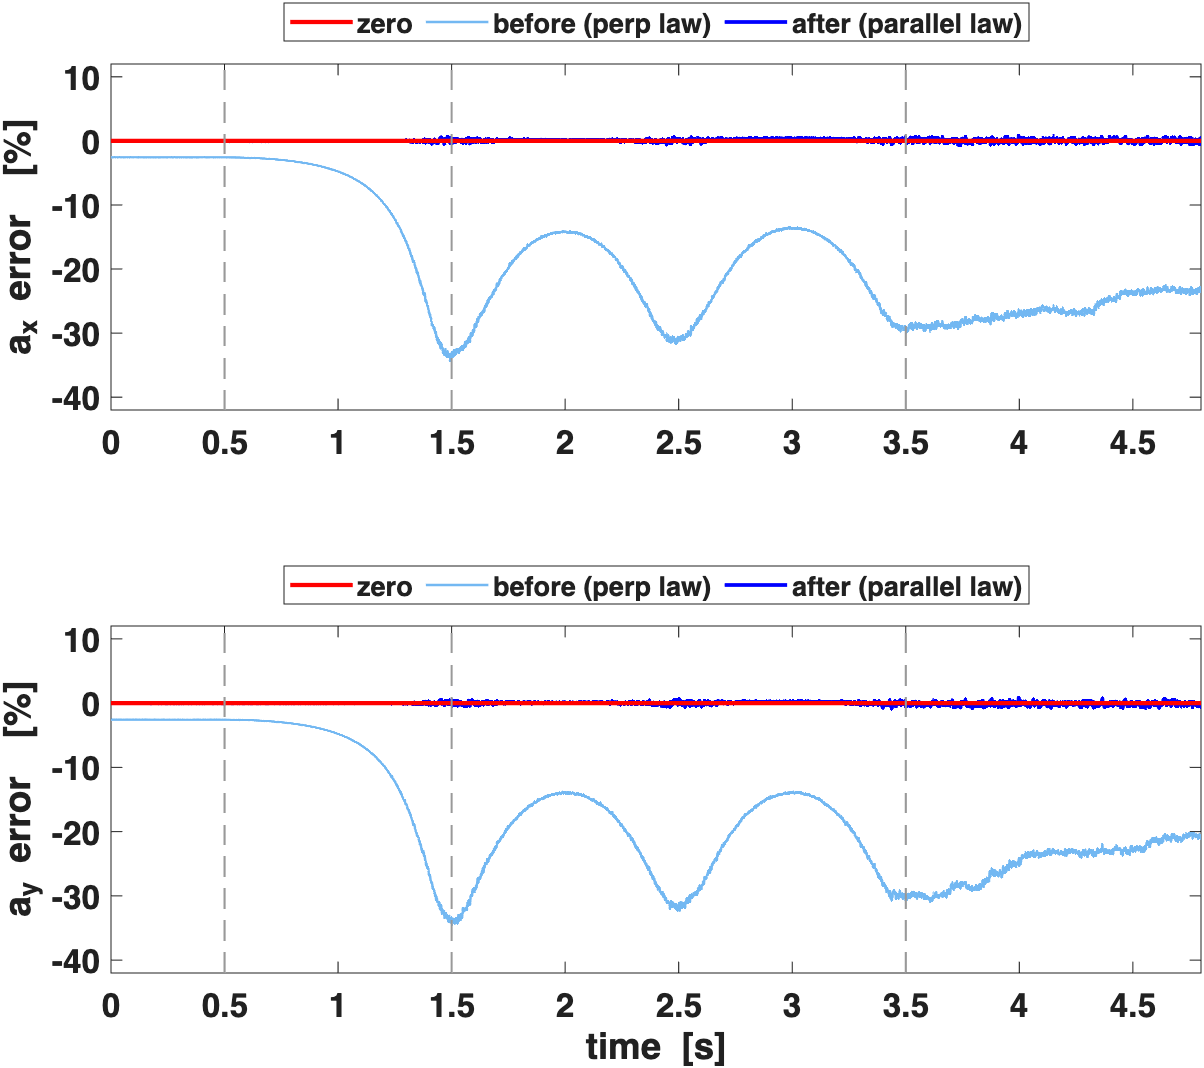
\includegraphics[width=0.49\linewidth]{figures/formB_c6_seed7.png}\hfill
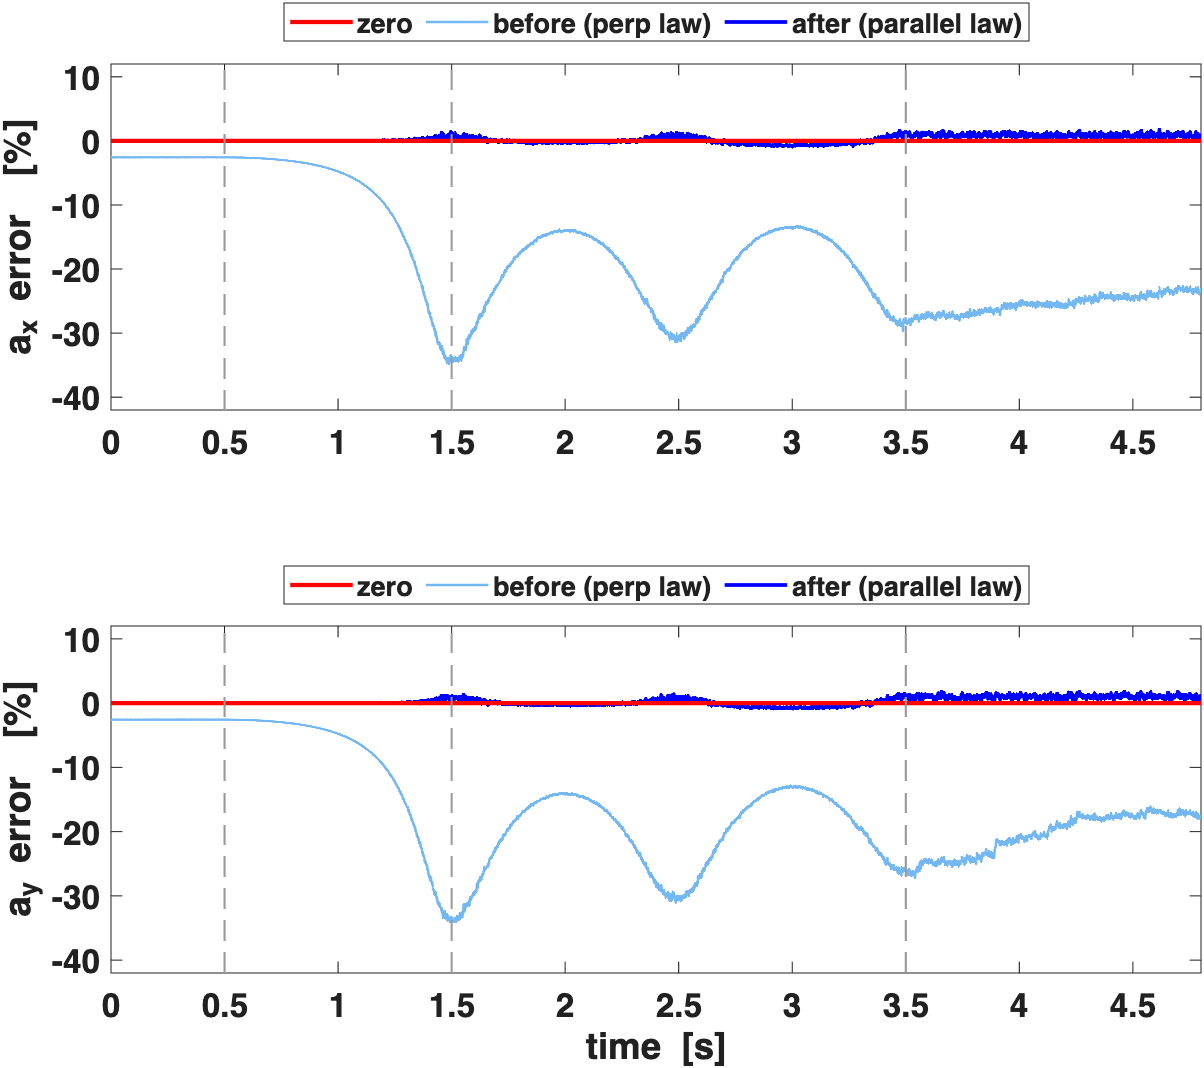
\includegraphics[width=0.49\linewidth]{figures/formB_c6_seed11.png}

Config 6 --- Stage 1a, $x/y$ gain estimation before (perpendicular law,
$b{=}9/8$) vs after (derived parallel law, S1 parallel block): 6-seed
means desc $34.8/34.1 \to 0.92/0.86\,\%$, hold
$-25.0/-22.6 \to -0.04/+0.01\,\%$; $z$ bit-identical.
Seed 7 (left) vs seed 11 (right).
\end{center}

\end{document}
